\chapter{Dataset}
\label{appendix:dataset}
\section{Dataset Collection}

\subsection{Ground Truth Data}
To measure accurate ground truth data, the RTAB-MAP application (Real-Time Appearance-Based Mapping) was used. RTAB-MAP is a Simultaneous Localization and Mapping (SLAM) framework that uses RGB-D, stereo, and LiDAR technologies, as well as graph-based incremental appearance-based loop closure detection. In general, SLAM involves emitting laser pulses, analyzing their return times, and generating 3D point clouds that represent the environment. The data can then be used to determine a subject's position and orientation. For more details, one can refer to the RTAB-MAP website \cite{rtabmap} and Wevolver's LiDAR SLAM article. \cite{malik_2023_lidar}
\par
The process of collecting ground truth data involved initializing RTAB-MAP on an iPhone, starting a new data recording session, and walking along the designated spiral path. To make sure that the recorded data was as accurate as possible, the phone's camera was kept unobstructed throughout the recording. RTAB-MAP's output, which is sufficiently accurate for this project, was used as the benchmark ground truth data.

\subsection{Sensor Data}
During the collection of ground truth data, the Arduino setup was activated, and the subject walked along the spiral path to collect raw sensor data. By integrating and processing the collected raw measurements, the subject's orientation and position were estimated. The Wi-Fi data was collected using a 2nd Arduino microcontroller, which exclusively scanned for RSSI values. The data was retrieved by the main Arduino module via a UART connection.

\subsection{Measurement Apparatus}
To simulate real-world conditions, measurements were conducted with the sensors attached to headphones, replicating their intended final placement. A custom measurement device (\cref{measurementapparatus}) was used to ensure accurate data collection. This device was then attached to the headphones as can be seen on \cref{measurementapparatus}. With this approach, the collected data accurately reflected the end-use scenario, making it reliable for realistic position and orientation estimation.

\begin{figure}[h] 
	\centering 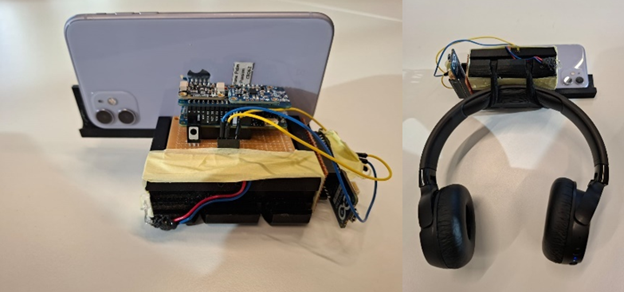
\includegraphics[height=4cm]{./images/apparatus.png}
	\caption{The 3D printed measurement apparatus.}
	\label{measurementapparatus}
\end{figure}

\subsection{Data Collection Process}
After setting up the measurement device, the data was collected. The data collection was done on the spiral of the GroupT campus in Leuven, Belgium. For each data recording session, the person wearing the measurement device must start and end the session at the same point, more precisely at the beginning of the spiral. In addition, the person stops at the same point, more precisely at the top of the spiral, before heading back to the starting position. Every measurement session lasts 10 minutes, but extending the duration can improve accuracy.
\par
Two types of measurements were taken. The first one represents an ideal sequence where the subject walks along the middle of the spiral in a straight line, with no interference, steady pace, and limited head rotation. The second type of measurement involves the person who is collecting data to walk along the spiral while applying more natural and random movements, such as moving up and down multiple times, moving the head in random orientations, moving away from the center of the spiral's path, etc. In total, 1 hour and 50 minutes of data was collected.

\section{Dataset Preprocessing}
After collecting our dataset, it had to be preprocessed in multiple ways before it was usable with our systems and evaluations. First of all, the data is sent from the Arduino to the desktop python environment where it's processed further.

\subsection{Synchronization}
Since the Arduino data and the ground truth data are running on two separate independently clocked systems, a synchronization step is required first. To do this, a computer vision-based synchronization mechanism was implemented. 
\par
As previously mentioned, both the raw data collection setup and the iPhone were mounted on a single measurement apparatus. An LED, connected to the Arduino, was positioned in the iPhone camera's field of view. Such LED lights up when the sensors connected to the Arduino are collecting data, serving as a synchronization marker. Using the OpenCV library, the irrelevant SLAM data that was recorded when the LED was off was filtered out. In addition, the sampling frequency of the raw data was much higher than the sampling frequency of the ground truth data, meaning that at the end of each recording session there were less ground truth samples than raw ones. Because of this, linear interpolation was used when necessary to match the oversampled raw data to the closest SLAM data points.

Furthermore, to improve the coarse synchronization's accuracy, a cross correlation was done over the initial ground truth orientation and measured orientation data, and the data was offset slightly in time to finely synchronize the measurements.
\begin{figure}[h] 
	\centering 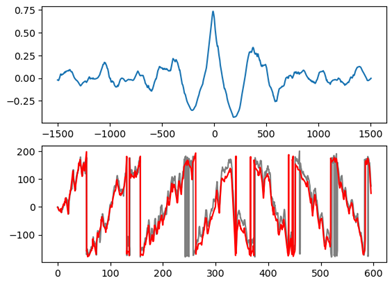
\includegraphics[height=4cm]{./images/crosscorrel.png}
	\caption{The results of the cross correlation of the ground truth and measured rotations (top) and the shifted data (red) after the delay was calculated (bottom).}
\end{figure}


\subsection{Alignment and Normalization}
Due to the inconsistent starting orientations and initial conditions, the ground truth data isn't always aligned to the same origin. In order to ensure our evaluation was valid, we implemented a data preprocessing step that ensures the entire dataset is aligned in 3d space. The implementation first ensures all the spirals are centered about the same point, and then aligns the starting points of the aligned spirals.

\begin{figure}[h] 
	\centering 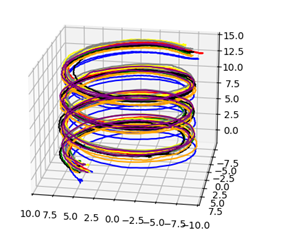
\includegraphics[height=5cm]{./images/aligned_data.png}
	\caption{The aligned spiral data.}
\end{figure}

After the alignment step, the sensor data is normalized so that the initial measurements are the "baseline values". Orientation data has the initial measurement subtracted from all measurements, resulting in it starting at the orientation origin. The ground truth orientation is similarly processed, however in quaternion space. Finally, the pressure data is preprocessed to remove outlier values due to sensor errors.

\section{Dataset Storage}
After synchronization, the data is stored so that it can be further processed. More precisely, the data was stored in HDF5 format (Hierarchical Data Format version 5). More precisely, the data for each full measurement session is stored in one HDF5 file which consists of the ground truth data, the raw data, and the Wi-Fi data. HDF5 format was used for data storage due to its multiple advantages such as its ability to store large datasets in structured hierarchy. The format is presented below.  \cite{hierarchical}
\par
\begin{table}[h!]
\centering
\renewcommand{\arraystretch}{1.1} % Reduce row height
\setlength{\tabcolsep}{8pt} % Reduce column spacing
\begin{tabular}{|l|l|}
\hline
\textbf{Group / Category} & \textbf{Subcategories} \\ \hline
\multirow{3}{*}{GT\_DATA}  & ORIENTATION            \\ \cline{2-2}
                           & POSITION               \\ \cline{2-2}
                           & TIMESTAMP              \\ \hline
\multirow{6}{*}{RAWDATA}   & 9DOF                   \\ \cline{2-2}
                           & BMP                    \\ \cline{2-2}
                           & BNO                    \\ \cline{2-2}
                           & PRESSURE               \\ \cline{2-2}
                           & RPY                    \\ \cline{2-2}
                           & TIMESTAMP              \\ \hline
\multirow{4}{*}{WIFIDATA}  & BSSIDS                 \\ \cline{2-2}
                           & COUNTS                 \\ \cline{2-2}
                           & RSSIS                  \\ \cline{2-2}
                           & TIMESTAMP              \\ \hline
\end{tabular}
\caption{Structure of an HDF5 file}
\label{tab:hdf5_structure}
\end{table}